\section{Processos}
O trabalho de coleta pode ser dividido em duas grandes partes, a coleta em si e a mineração de dados. Uma parte dessa mineração é feita inteiramente automatizada usando algoritimos e bibliotecas, entretando, existe outra parte que envolve a entrada de dados especialistas.

Nessa sessão séra dado um pequeno detalhamento de como funciona a coleta e a mineração, e como foi utilizado as ferramentas préviamente citadas nesse trabalho. Será iniciado o detalhamento pela coleta, uma vez que é necessário existir algum dado para que seja possível qualquer outra ação


\subsection{Coleta}
Para isso existem ainda algumas configurações pendentes, como podemos observar na figura \ref{fig:creds}, existem duas telas, a primeira é o \textit{dumont/sample\_env} e a segunda a réplica criada anteriormente \textit{dumont/dev.env}, foi removido todas as variáveis referentes aos serviços da AWS, já que não será utilizado local como já abordado, além disso foi retirado o usuário e senha do mongo já que o serviço no docker foi configurado para não precisar do mesmo. Além disso a variável \textit{COLLECTOR\_REQUEST\_TOKEN} pois a intuição dela é criar um mínimo de autenticação caso utilize essa API pública na internet. Por fim o \textit{COLLECTOR\_LIMIT} irá limitar a quantidade de usuarios a serem coletados a cada requisição.

\begin{figure}
    \centering
    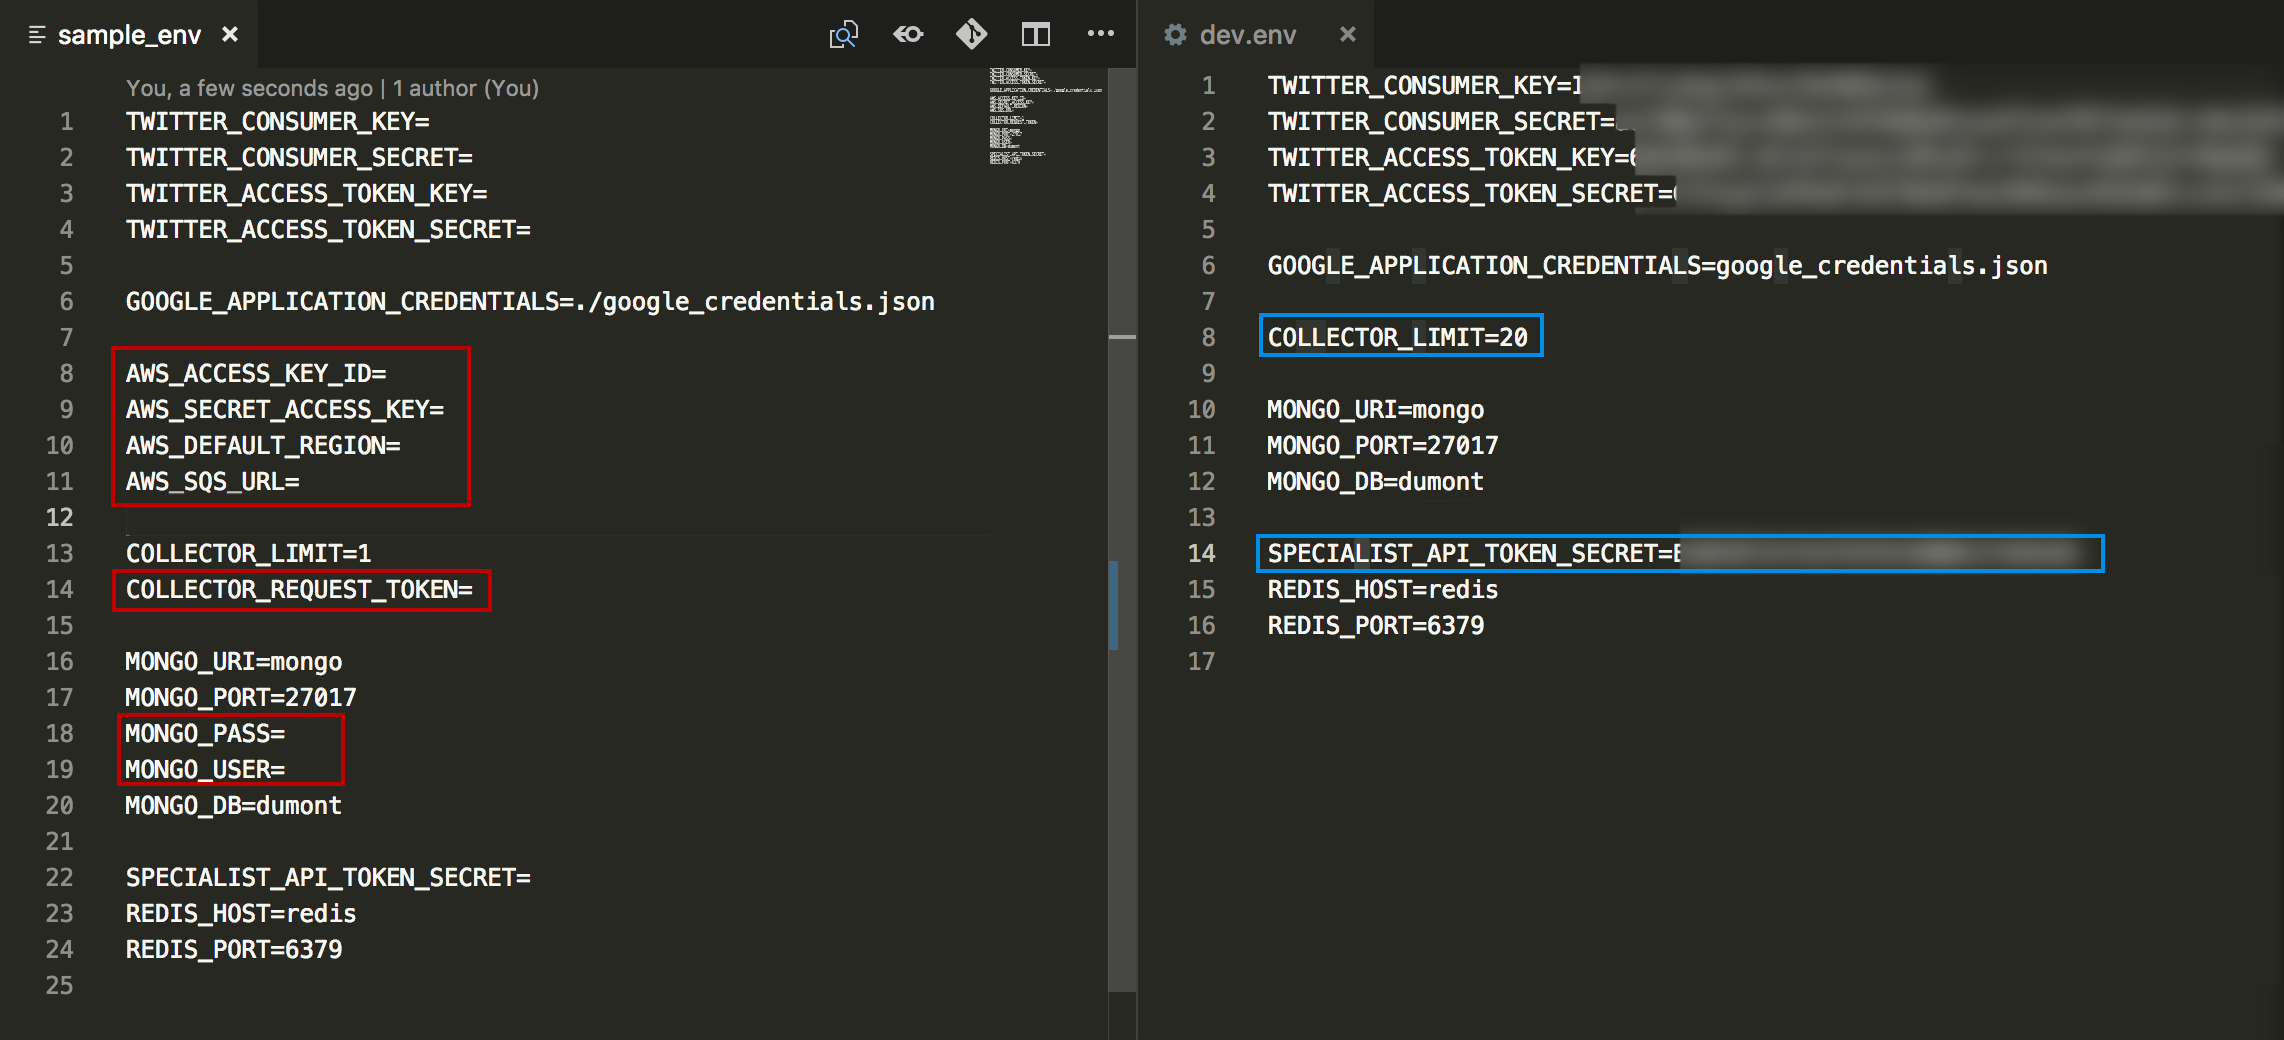
\includegraphics[width=1\textwidth]{imagens/creds.png}
    \caption{Imagem demonstrando passo a passo de como gerar o JSON de credencial}
    \label{fig:creds}
\end{figure}

É importante lembrar dos limites da API publica do twitter, e tambem que devido a implementação (que pode ser acompanhada no arquivo \textit{dumont/collector/twitter/index.js}) na linha 74 é possível ver o momento onde a \textit{stream} é parada, entretando, podem chegar inumeros tweets de diferentes usuarios simuntaneamente, fazendo assim, com que sobrecarregue a quantiadade de usuarios permitidas na API. É sugerido rodar valores baixos entre 20 a 45 para evitar problemas.

Uma vez configurado, é possivel executar o comando \textit{docker-compose -f docker-compose.dev.yml}, uma vez que o docker inicie o serviço você pode iniciar a coleta utilizando desde um navegador, ferramentas (um exemplo é o Postman\footnote{https://www.getpostman.com/}) ou até mesmo o \textit{curl} utilizando o uri \textit{\url{http://127.0.0.1:8080/}}

Depois que os dados foram coletados, ja é possível minerar algumas informações deles, para isso existem processos a serem detalhados.
\subsection{Mineração}
O segundo passo após coletar os dados é rodar scripts de mineração. Uma das maiores dificuldades é como manipular os dados de maneira incremental. Desde que a pesquisa teve inicio, muitas ideias surgiram, novos pontos de vistas e novos dados a serem minerados. Foi adotado uma propriedade chamada \textit{processing_version}, essa propriedade marca o documento com a versão do processamento dele.

Dentro da pasta \textit{dumont/tasks/processing} existe duas pastas, uma para processar usuários e outra para processar tweets, ambas exportam vários estágios de processamento, esse estágio é exportado e passado para uma classe chamada \textit{Processor} localizada no arquivo \textit{dumont/tasks/processing/__init__.py}, o nível de processamento base é o 0 (nível inserido na hora que o coletor salva do dado no banco), a partir disso é possível atualizar o processamento por um script (no caso existe a possibilidade de consumo da fila, porem, como já dito essa abordagem esta contida no anexo 1).

Quando o coletor foi configurado, automaticamente todos os dados necessários para o processamento já foram preenchidos. A tarefa de processamento é responsável por:

\begin{itemize}
    \item Remoção de \textit{stop-words}: Existem palavras que prejudicam a analise textual por não serem essenciais ou estarem colocadas de maneira equivocada. Um dos processos retira esse tipo de ruído do texto.
    \item Arvore Léxica: Criar uma arvore léxica baseada na frase original do tweet e na frase que já foi tratada removendo as \textit{stop-words}.
    \item Analise de Sentimento: Utilizando a API do Google Language é retirado o sentimento da frase original e da frase tratada também.
\end{itemize}

Para obter esses dados basta rodar o comando \textit{docker-compose -f docker-compose.dev.yml up tasks}. Com esses dados já é possível ter alguma noção de informações relevantes dos textos, porém ainda é necessário de embasamento técnico, ou seja, um dado especialista que possa orientar a máquina a utilizar as demais propriedades mapeadas para localizar um delta em comum.

Existe um outros serviços contidos dentro do projeto o \textit{dumont/specialist-api} e \textit{dumont/specialist-app} que gera uma API e uma interface gráfica para injeção de dados especialistas. Para subir ambos os serviços basta utilizar o comando \textit{docker-compose -f docker-compose.dev.yml up specialist-app}. Entretanto, é necessário de um usuário para injetar as analises, é possível criar o documento na mão dentro do mongo, porem, existe um binário dentro da pasta chamado \textit{dumont/create\_specialist}, basta executa-lo passando o e-mail e ele te devolvera uma senha aleatória. Então basta acessar \textit{\url{http://127.0.0.1:3000/}} e utilizar os dados para entrar no sistema. Logo que autenticado você encontrara uma tela igual a da figura \ref{}, nela existe o tweet, uma área para adicionar perguntas da EADS relacionadas, e um local onde pode-se identificar palavras chaves dentro daquele tweet.

Com o sistema rodando, e dados sendo coletados e analisados é necessária uma amostragem para melhor assertividade e desenvolvimento. Durante a pesquisa, em uma preliminar foram coletados mais de 160GB de dados. A amostra foi tirada antes mesmo da inserção de dados especialistas, logo é necessário conhecer os \textit{scripts} de seleção do dumont.

